\chapter{Theoretical Framework}
\label{ch:theoretical-framework}

Before starting with rehabilitate the main topic, some basic concepts, technical terms and underlying theory has to be explained.
This is important to faster read through the thesis without the need to interrupt the flow of thought.
In the following, a set of established theories and terms is explained which are not directly related to the thesis formulation, but essential to comprehend numerous contexts.

\section{Android UI}
\label{sec:android-ui}

To be able to use any of the things displayed on the mobile device, some concepts of \gls{ui} programming must be shown.
A \gls{ui} enables the user to view the applications data on the screen but also to interact with the device especially on mobile devices \cite{android_ui_layer}.

The main challenge is to bring the application data in the right format, so that the display can interpret the instructions to draw the elements.
Each mobile phone with the Android \gls{os} has a basic set of native functions through which the \gls{ui} can be drawn and updated, a so-called \gls{api}.
These functions can be very general to instruct drawing a whole component such as an alert box, or they can be very specific as drawing single rectangles in a canvas.

The rough transition from the application data (data layer) to the display data (ui layer) is depicted in figure \ref{fig:android_udf}.
The application data is transformed, concatenated or filtered to be saved in a view model, which represents the state for each view.
The view model is then layed out to multiple \gls{ui} elements.
E.g.\ they are loaded in the Android activity via view layouts~\cite{android_draw_views} or composed in a declarative approach~\cite{android_jetpack_compose}.
It is generally advised to use a \gls{udf}.
This ensures that the data is only changed in one place and doesn't get out of sync between \gls{ui} elements, the view model and the data layer.
The \gls{ui} can also register user inputs (like a button press) and report them back to the view model.
The view model then updates the application data, if needed, and then also reports the current \gls{ui} state back to the UI elements to be rerendered.

\begin{figure}[htbp!]
    \centering
    \begin{subfigure}[b]{0.5\textwidth}
        \centering
        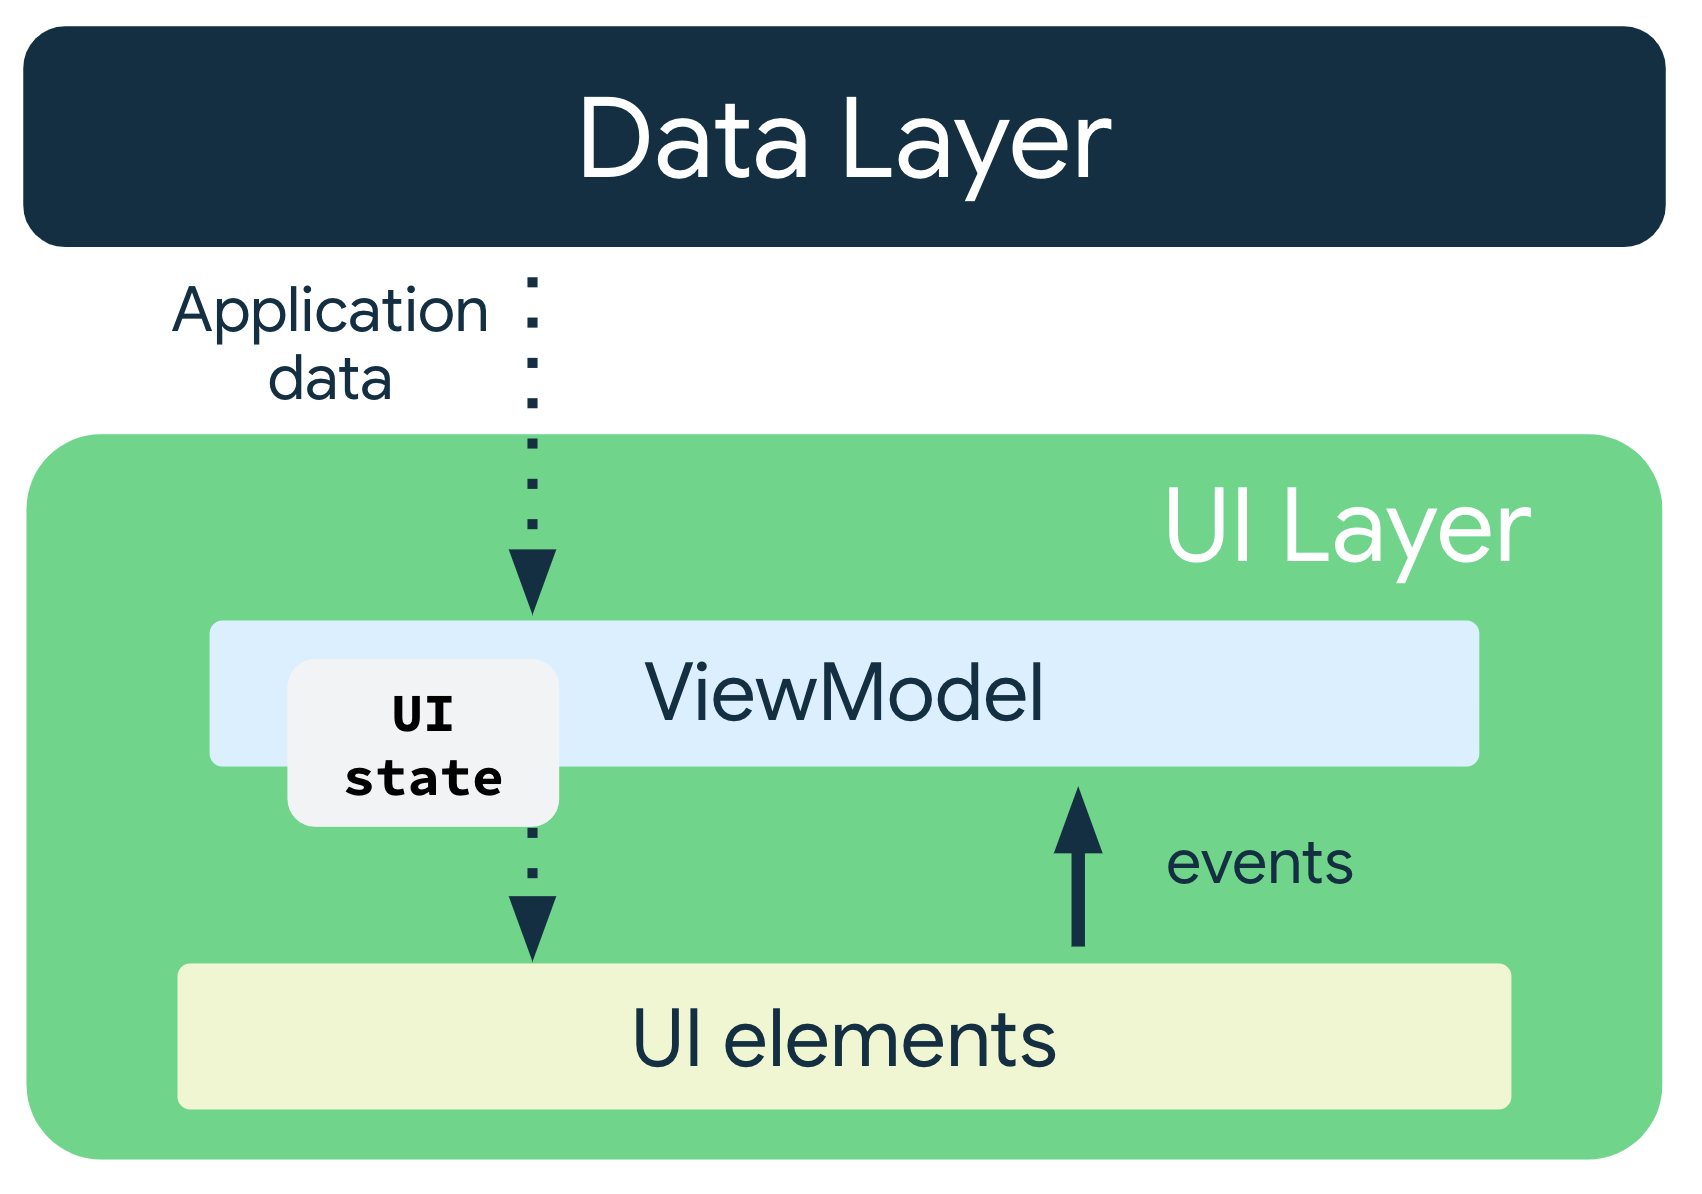
\includegraphics[width=\textwidth]{graphics/android_udf}
        \caption{Diagram of \gls{udf} in app architecture \cite{android_ui_layer}}
        \label{fig:android_udf}
    \end{subfigure}
    \hfill
    \begin{subfigure}[b]{0.4\textwidth}
        \centering
        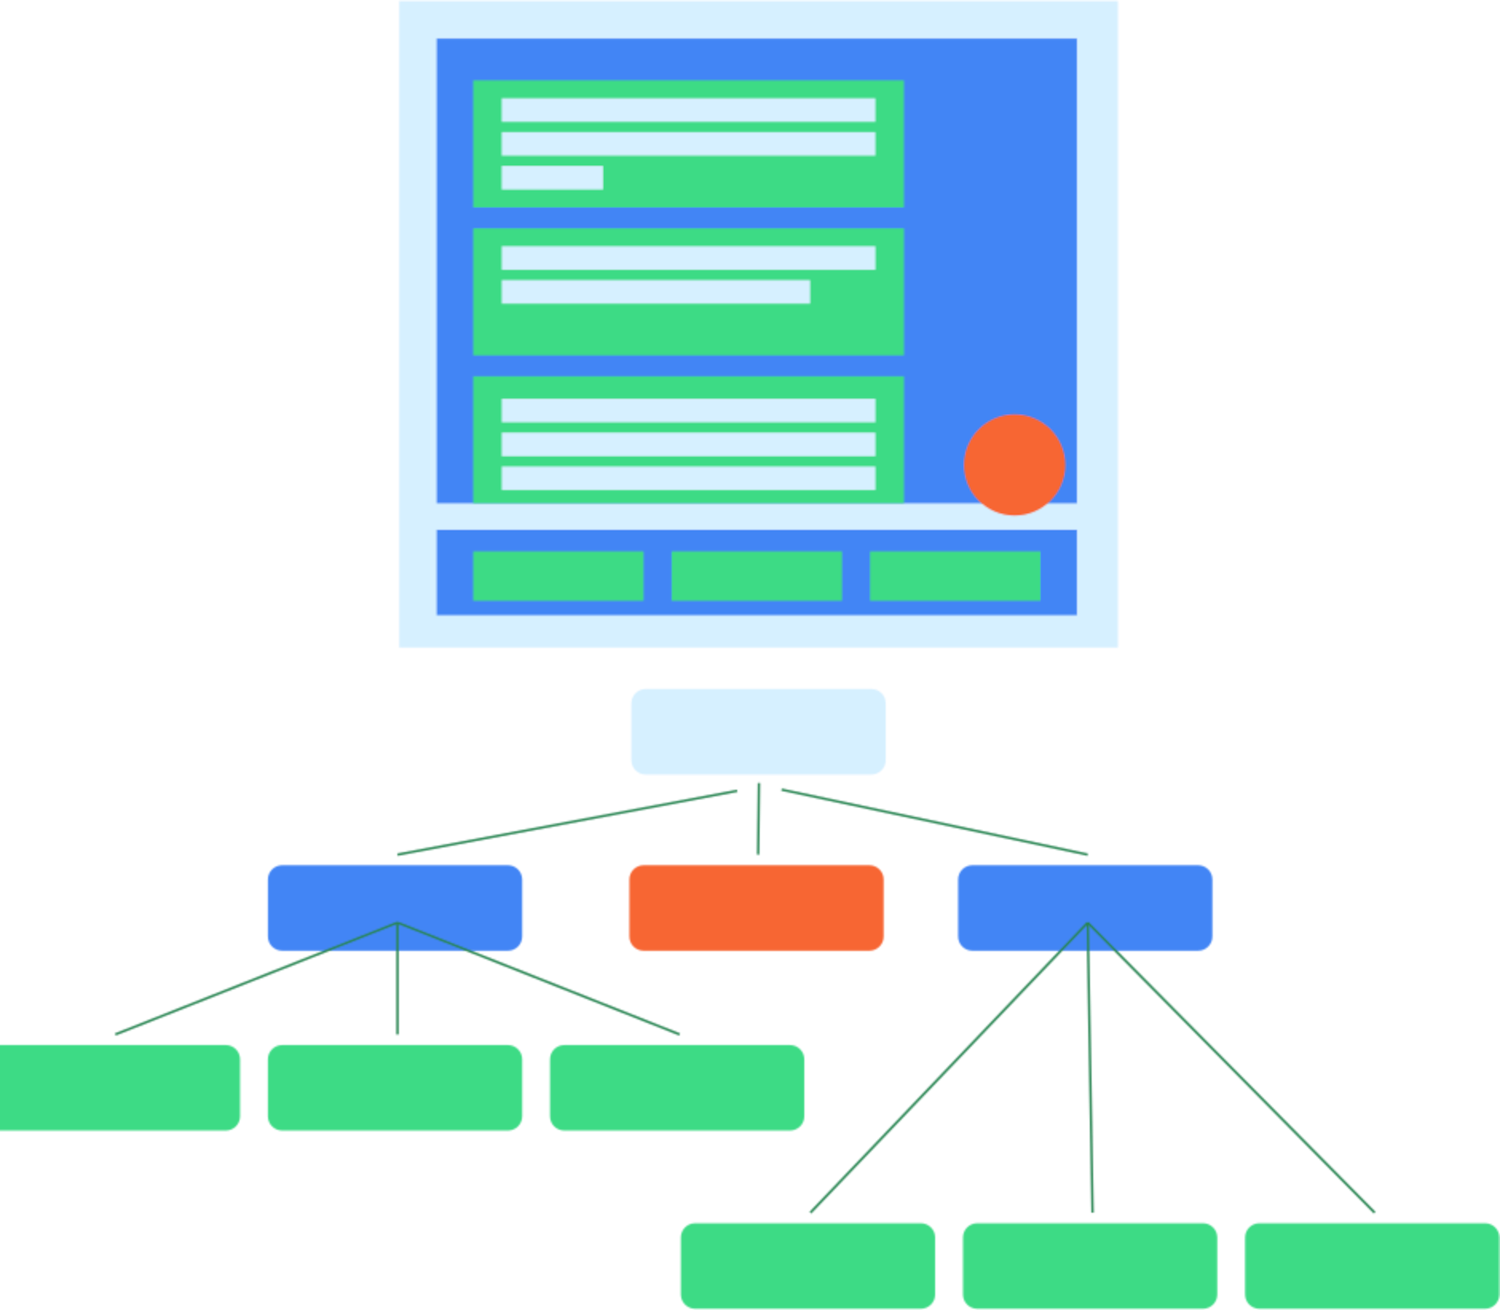
\includegraphics[width=\textwidth]{graphics/android_semantics-ui-tree}
        \caption{Schema of how the semantics tree is related to the \gls{ui} hierarchy \cite{android_semantics_compose}}
        \label{fig:android_semantics_ui_tree}
    \end{subfigure}
    \caption[Structure of the Android UI]{Structure of the Android \gls{ui}}
    \label{fig:android_tree}
\end{figure}
%https://developer.android.com/guide/topics/ui/how-android-draws \cite{android_draw_views}
%https://developer.android.com/jetpack/compose/mental-model \cite{android_jetpack_compose}

\subsection{Data Tree Structure}
\label{subsec:data-tree-structure}

The \gls{ui} elements (i.e.\ the composition) themselves are hierarchically structured in a tree.
This allows the renderer to calculate relative distances, floatings and skip processing hidden or overlapped elements.

With the Android Layout Inspector (figure~\ref{fig:android_layout_inspector}) a view hierarchy tree can be visually inspected while displaying its position and layout on the Android screen.
Also, the layout attributes can be validated.
This tool allows to debug complex \gls{ui}s especially when using nested components and display them in a simplistic way.
Note that this tool is only available if one has access to the app's source code.

\begin{figure}[htbp!]
    \centering
    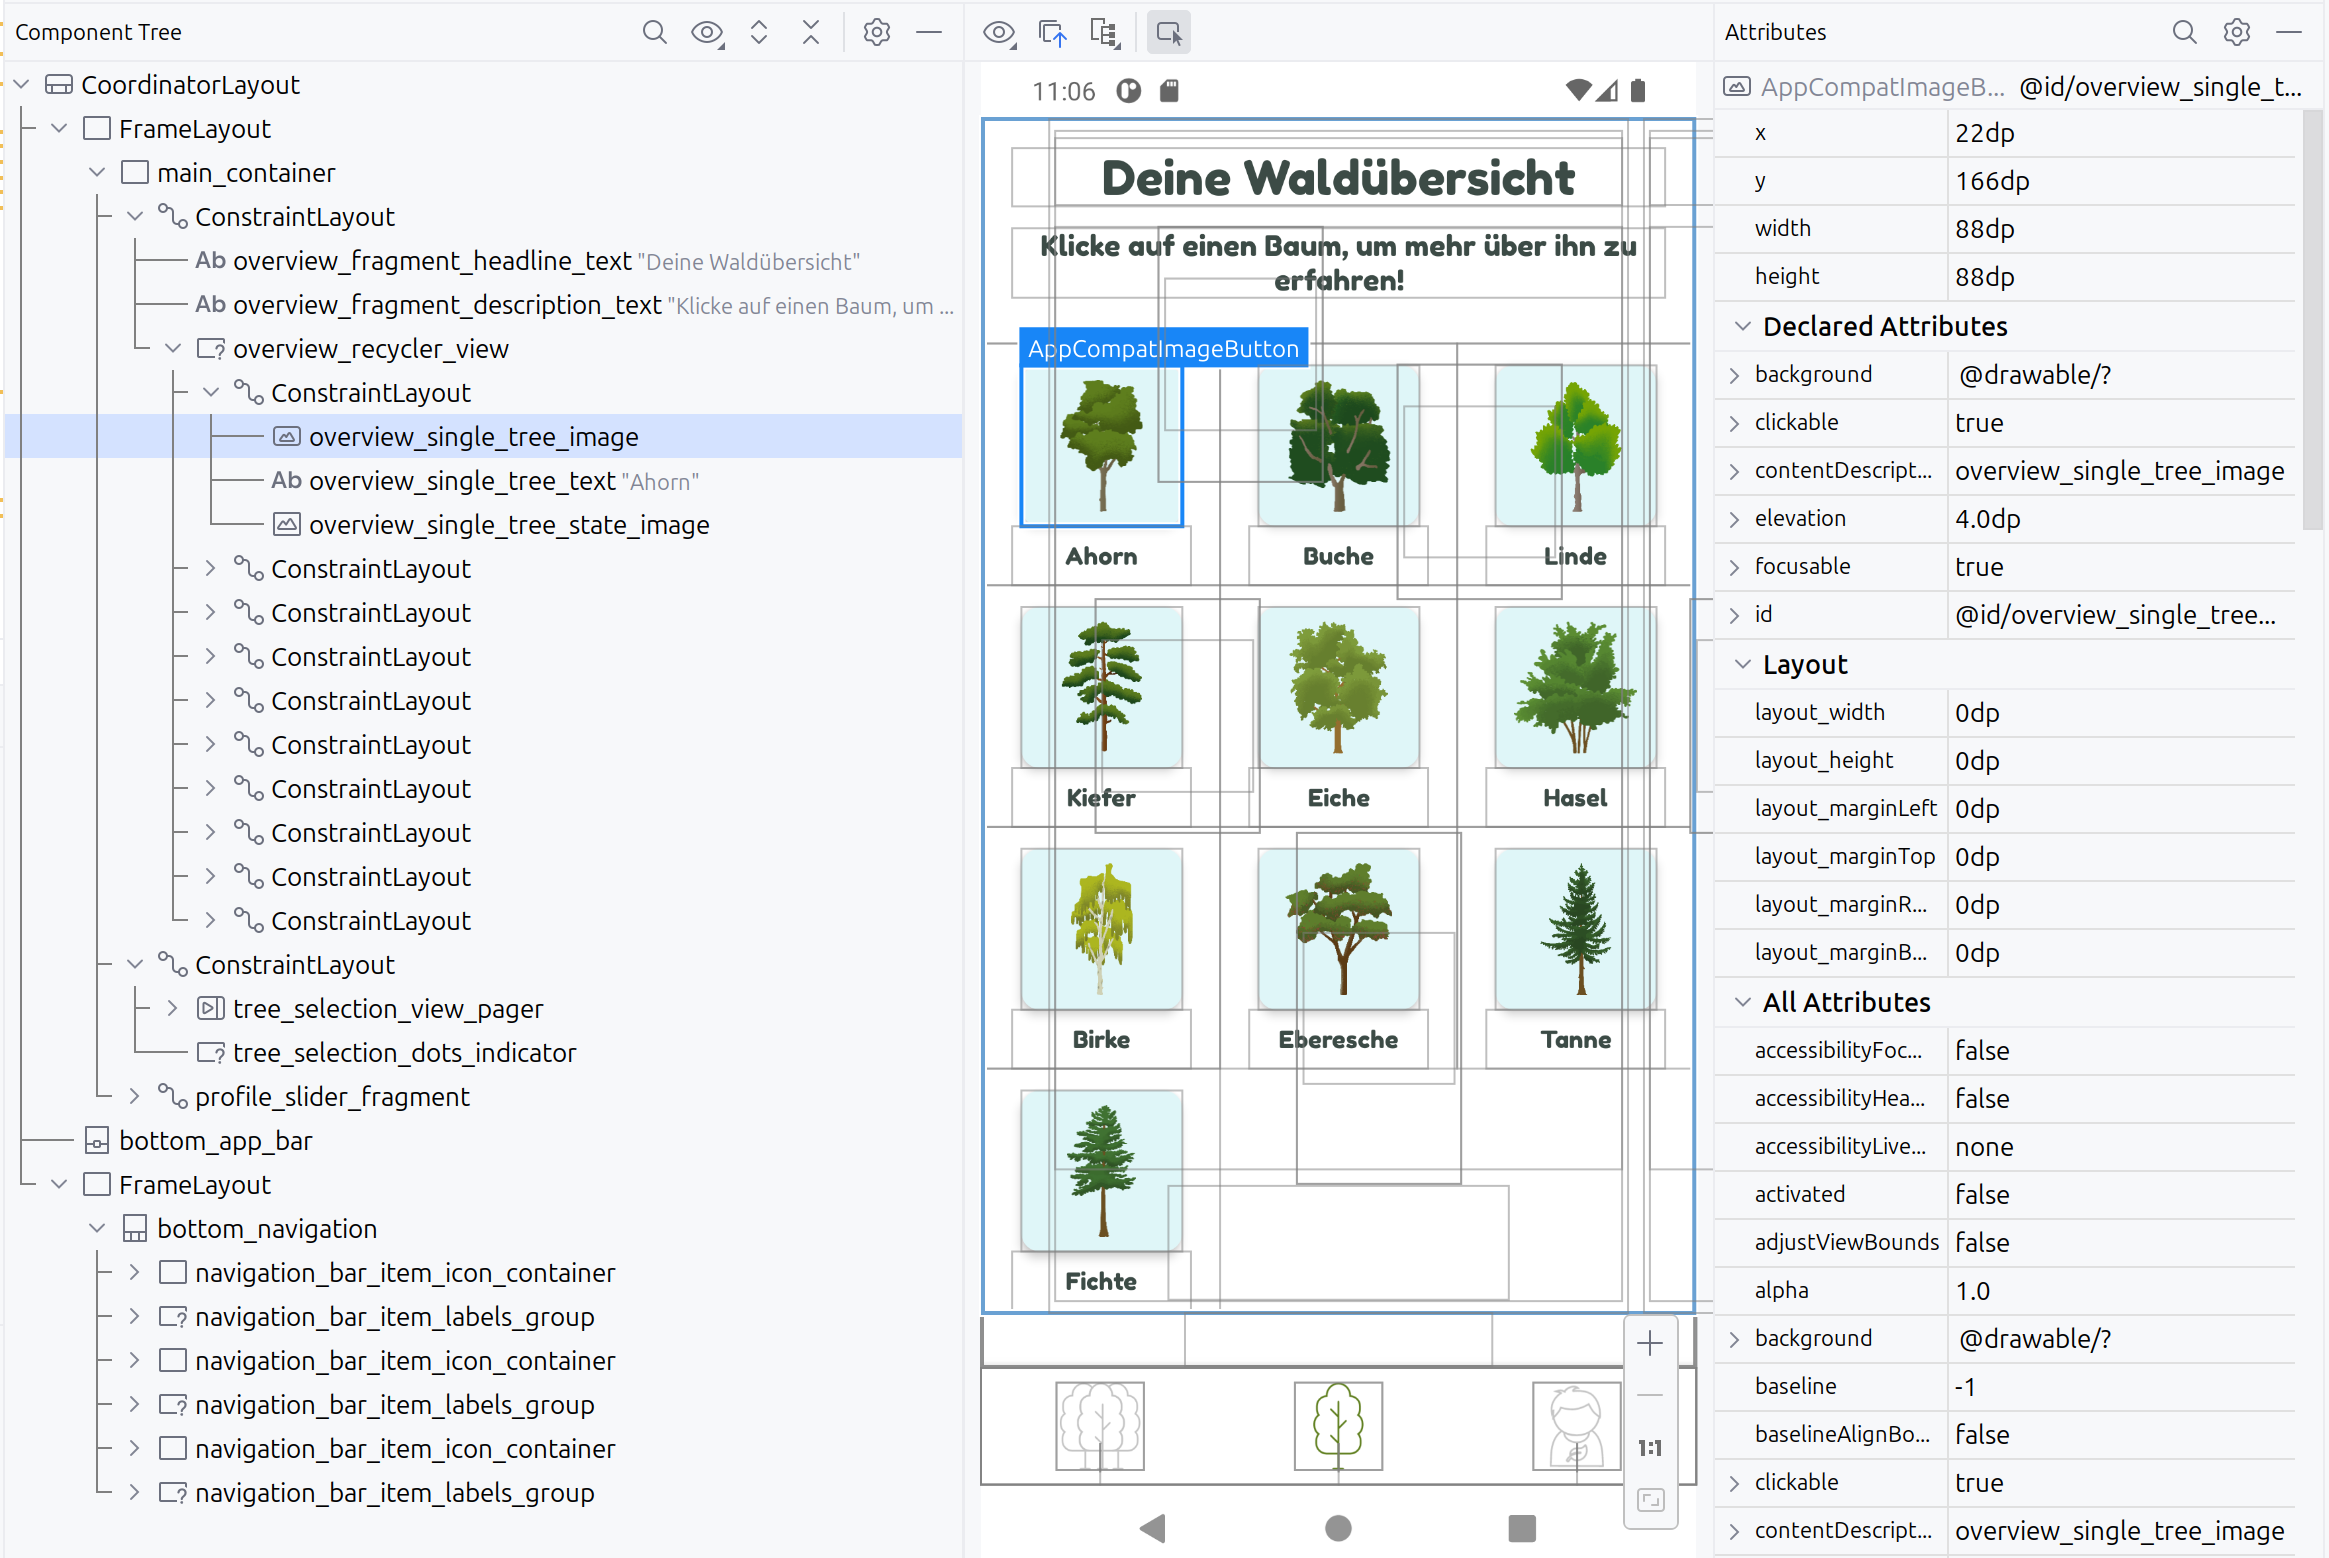
\includegraphics[width=\textwidth]{graphics/android_layout_inspector}
    \caption[Android Layout Inspector tool]{The Android Layout Inspector tool using the example of \quotes{App ins Grüne}~\cite{mimuc_app_ins_gruene} by the Media Informatics Group of the LMU in Munich.}
    \label{fig:android_layout_inspector}
\end{figure}

\subsection{Android Accessibility Service}
\label{subsec:android-accessibility-service}

If an app is running in production on a users device, meaning that the app is compiled and publicly available, the ways of accessing the Android \gls{ui} tree are limited.
This behavior is of course wanted for safety and privacy reasons.
Nonetheless, if desired, a user can explicitly allow certain apps to gain access to the semantics tree of your Android \gls{os}.
This is especially useful for providing accessibility services for impaired users (like done with the TalkBack app).
Or, as in our case, the setting can be used to enable services which collect data for user studies or scientific experiments.

This semantics tree is deviated from the existing \gls{ui} tree.
It can be fed via special semantic properties while composing the \gls{ui}, e.g.\ by specifying the \code{contentDescription} property of an icon \cite{android_semantics_compose}.
Providing semantics is not limited to native platforms as shown by Flutter~\cite{flutter_semantics} and React Native~\cite{react_native_accessibility}.
In figure~\ref{fig:android_semantics_ui_tree} a schema is presented, which shows how the elements of the semantics tree are spanned compared to the components on the \gls{ui} layer.

%https://github.com/android/codelab-android-accessibility
To take advantage of the semantics tree, a custom accessibility service can be built, which can run in the background.
This service tracks all UI changes and has access to the current view hierarchy of the screen, which also inherits the semantic tree.
By altering the code of the \ti{AccessibilityNodeInfoDumper} one can extract the view hierarchy to a locale or remote database~\cite{android_accessibility_node_info_dumper}.
In the code section \ref{android_accessibility_node} a small fraction of a view hierarchy is shown.
It contains nested nodes with various attributes which represent the components of the combined \gls{ui} and semantics hierarchy.

%Semantics tree:
%https://api.flutter.dev/flutter/widgets/Semantics-class.html
%https://developer.android.com/jetpack/compose/semantics
%https://android.googlesource.com/platform/frameworks/testing/+/jb-dev/uiautomator/library/src/com/android/uiautomator/core/AccessibilityNodeInfoDumper.java \cite{android_accessibility_node_info_dumper}
%https://github.com/Gustl22/android-accessibility/blob/c158808533d6fc017455184a7317555d3e6946f6/GlobalActionBarService/app/src/main/java/com/example/android/globalactionbarservice/uiautomator/AccessibilityNodeInfoDumper.java

%Mean 18 actionable elements, with Std=12. \cite{zhou2021large}

\lstinputlisting[language=XML,label=android_accessibility_node,caption={Android Accessibility Node in XML.},float]{code/android_accessibility_node.xml}

\section{Machine Learning}
\label{sec:machine-learning}

\gls{ml}, a term spread by Arthur Lee Samuel, is a method of data analysis, more precisely a scientific approach to form statistical models without the need to explicitly program it~\cite{mahesh2020machine}.
It uses algorithms to iteratively learn how data is structured.
In contrast to statistical inference or manually crafted statistical models respectively, \gls{ml} can solve tasks by automation of model building.
Its advantages lie in finding hidden relations and patterns from the context, without having any or only a small pre knowledge of the data, thus it is a strong tool for generalization or abstraction of large datasets, also known as \Gls{gl-bigdata}.
\gls{ml} can be applied to the following fields among others: email and spam filtering, fraud detection, cybersecurity, web search engines, recommender systems (like known from Netflix or Amazon), advertising, translators and text generation, pattern and image recognition.
The data driven approach also comes with some drawbacks: the outcome heavily depends on the provided data.
It can include biases and therefore may acquire forms of discrimination or unfair treatment.
Nonetheless \gls{ml} has a lot of potential to uncover hidden connections in large datasets.
The most important concepts are explained to be able to follow certain decisions in this thesis.

%\todo{explain Tensors, Datasets}
%https://stackoverflow.com/a/48599383/5164462

\subsection{Preprocessing}
\label{subsec:preprocessing}

Preprocessing describes the step after one acquired their data, but before training the \gls{ml} model.
This step is not to be underestimated.
A \gls{ml} model can perform significantly better when certain preprocessing steps are applied \cite{alam2019impact}.

To be able to preprocess, we have to know with what kind of data we handle with.
Data entries can occur in different forms, but we can break them down in three main types:
\begin{itemize}
    \item \tb{Categorical values}: a value is always assigned to a class with a fixed pool of predetermined classes.
          E.g.\ letters, words, brands, animals, chemical elements
    \item \tb{Continuous values}: the value can be fractional and may lies in between a lower and an upper bound.
          E.g.\ temperature, velocity, geographic position
    \item \tb{Integer values}: the value is a whole number and may also lie in between a lower and an upper bound.
          E.g.\ revolutions per minute, product number, annual sales
\end{itemize}

For all types -- discrete, continuous, and categorical values -- we have a wide variety of options for preparing them in order to be subsequently processed by a \gls{ml} model \cite{duong2021}.
These are listed in the following, while not all can be applied to all types of values.

\subsubsection{Feature Selection}

Feature selection is a crucial step to successfully develop a model with the desired results.
It can improve learning performance, thus reduces time, increases computational efficiency, decreases memory storage, and helps build better generalization models \cite{li2017feature}.
Also, it may be a valid approach to get around missing data and can help structure the data by removing unnecessary clutter.

%https://dl-acm-org.emedien.ub.uni-muenchen.de/doi/pdf/10.1145/3136625
On the technical sight, feature selection can be differentiated for two goals: supervised and unsupervised learning~\cite{li2017feature} (cf. section \ref{subsec:machine-learning-types}).
However, principles from the supervised feature selection can be applied in the unsupervised domain, resulting in a semi-supervised filter selection.
For classifiers and regression problems (unsupervised) following methods can be applied.
Multiple features can be compared by calculating their correlation.
If one feature is uncorrelated to all other features, this may be an indicator that this feature can be dropped, as it doesn't contribute to the resulting model (\ti{filter method}).
However, this can only be stated for linear correlations, thus it can contribute to the result in an unpredicted way.
Also, if two features correlate too much to each other, one feature probably is redundant and can be dropped.
A good approach is also to reduce the dimensionality of the input data, e.g.\ by replacing~\gls{gl-one-hot} encoded features of the same domain with embeddings (\ti{embedded method}).
This is also called \ti{feature extraction}.
Feature extraction can also be used in unsupervised feature selection.
Clustering is a common approach to reduce the number of input dimensions by gaining insights of which classes can be merged and which need to stay.
A more computational but promising solution is to filter the features by optimizing the model result, also called a \ti{wrapper method}.
By gradually removing and adding features and calculating the models performance, one can determine which inputs are important and which are at risk to increase computing time without noticeable effect.

\subsubsection{Missing Data}
Some data entries may are missing.
Therefore, two approaches can be employed to get around these missing values.
First, one can drop these values by removing the column or row.
This is only recommended if you are not relying on this data entry, or this the whole feature is not expected to be important enough to bring any value to the model's performance.
Second, the data can be filled with a default value like zero or calculate a reasonable value from the surrounding data entries by taking their \quotes{mean, median, or interpolation}~\cite{duong2021}.

\subsubsection{Normalization and Standardization}

Many \gls{ml} models work better or exclusively with normalized data.
This means that the values have to be in a certain range, most commonly are from \tb{0} to \tb{1} or from \tb{-1} to \tb{1}.
This can be achieved by dividing all values with the difference of the minimum and maximum value and shift the output accordingly \cite{duong2021}.

% X new = (X — X min)/ (X max — X min)

Sometimes this is not enough, e.g.\ if having a few extreme values, and an approach is desired which better reflects the average data.
Here the standardization, also called z-score normalization, is applied.
This method scales the values so that the mean value is placed at \tb{0} and the standard deviation is placed at \tb{1}.
%https://medium.com/analytics-vidhya/what-are-data-standardization-and-data-normalization-f880dd9e79b6

\subsubsection{Padding}
\label{subsubsec:padding}

Padding is a technique to adapt input sequences or matrices of different dimensions to the same size.
For example if one screen only has five \gls{ui} elements, and the next one has twenty, the input size varies significantly.
Therefore, there exists three approaches to overcome this problem~\cite{baeldung_padding}.
The first one is to extend all inputs of a specific feature to the longest available input dimension of this feature.
Then every sequence has to be filled with additional values, almost always \tb{0} is used for that, until it matches the longest dimension (\ti{same padding}).
Another technique called \ti{valid padding} cuts all data values after reaching the smallest dimension of all inputs of the feature.
One can also use a combination to e.g.\ pad all inputs with zero to the mean dimension, but throw away all exceeding values as they aren't expected to contribute to a better result.
\ti{Causal padding} is a form of \ti{same padding}, but it prepends the fill values in front of the sequence.
This is helpful if having \gls{rnn}s, which rely on a lengthier inputs in order to predict their next value, without need of filtering out short sequences.

\subsubsection{One-Hot-Encoding for Categorical Values}
\label{subsubsec:categorical_variables}

A categorical value must be treated differently than numerical ordinal values.
This is demonstrated best on a concrete example.
Imagine a dataset with pictures of animals, and we want to categorize their species.
Then the values of all possible species like \code{dog} and \code{cat} is called \ti{vocabulary}.
To write it in a table, one could add a column called \code{species} and write their species as a \ti{string} (cf.\ table~\ref{tab:raw_data_table}).
Unfortunately a \gls{ann} cannot work with \ti{strings}, but only with numerical values.
So one could think that mapping each species to a number can solve this issue.
Indeed, this is possible for ordinal categories, which have a strict linear order, such as ratings or gradings.
They are then treated the same as \tb{integer values}.
But animals aren't structured ordinal, thus each species must be treated equally.
To reflect that we split the species column in multiple sub-columns, so that each new one represents one species, see table~\ref{tab:one-hot}.
If the animal belongs to that species, one inserts a \tb{1} or \tb{True} and if not, a \tb{0} or \tb{False} is filled.
This is also called \gls{gl-one-hot}-encoding ~\cite{brownlee2021}.

\begin{table}[htbp!]
    \begin{subtable}[c]{0.5\textwidth}
        \centering
        \begin{tabular}{|l|l|l|}
            \hline
            \tb{$I_{d}$} & \textbf{Img} & \textbf{Species} \\
            \hline
            0 & \ti{blob} & cat \\
            1 & \ti{blob} & dog \\
            2 & \ti{blob} & cat \\
            3 & \ti{blob} & horse \\
            \hline
        \end{tabular}
        \subcaption{Raw data table}
        \label{tab:raw_data_table}
    \end{subtable}
    \begin{subtable}[c]{0.5\textwidth}
        \centering
        \begin{tabular}{|l|l|l|l|l|}
            \hline
            \tb{$I_{d}$} & \tb{Img} & \tb{Cat} & \tb{Dog} & \tb{Horse}\\
            \hline
            0 & \ti{blob} & 1 & 0 & 0 \\
            1 & \ti{blob} & 0 & 1 & 0 \\
            2 & \ti{blob} & 1 & 0 & 0 \\
            3 & \ti{blob} & 0 & 0 & 1 \\
            \hline
        \end{tabular}
        \subcaption{One-hot encoded species}
        \label{tab:one-hot}
    \end{subtable}
    \caption[One-hot-encoding of categories]{\Gls{gl-one-hot}-encoding of categories, $I_{d}$ is the index of the data entry}
    \label{tab:cat_one_hot}
\end{table}

\subsection{Types of Machine Learning}
\label{subsec:machine-learning-types}

To get be able to evaluate which subfield of \gls{ml} is the best choice, we need an overview of the existing approaches listed in \cite{ghahramani2003unsupervised}.

\tb{Supervised Learning} is used for \ti{Classification} and \ti{Regression} tasks.
It uses \ti{labeled} samples, which means the input $x$ and output $y$ is known beforehand.
Essentially it learns through comparing the actual output (labels), which is provided, with the output the model \ti{predicts}.

Unlike in Supervised Learning, \tb{Unsupervised Learning} isn't provided any labels $y$.
It is used for clustering, dimensionality reduction or anomaly detection. %may need to explain more
E.g.\ in clustering the \gls{ml} model detects similar objects and groups them together.
What is seen as similar is up to the model, so it is not known before, with what groups or clusters the model comes up with.

The algorithms using \tb{Semi-supervised Learning} seek to adopt from unlabeled and labeled data~\cite{van2020survey}.
E.g.\ for a classification problem, the model is either trained first with unlabeled data resulting in clusters, which are then provided a class with a few labeled samples.
Or classes are trained based on labeled data, but their class boundaries are extended through unlabeled data, which follows the approach of clustering.
%It can be assumed that the model is trained first with labeled data, e.g.\ to be able to differentiate certain clusters.
%Then the model predicts the labels of the unlabeled data which is then serving as new data point to train the model.
%This helps to enlarge the cluster or move its boundaries.
%Test points to be classified by the model into the clusters then have a smaller distance to the previous predicted point,
%and therefore adapting the label of it's cluster, instead of being assigned to a different cluster.
%It can be seen as a model trained with classification through labeled data and then extended with clustering through unlabeled data.
%Also, if having only few labeled points, one can start with training a cluster through unlabeled data and then determine the class label of the clusters with the labeled data points.

%\tb{Self-supervised Learning}
%\todo{may explain Self-supervised learning}

\tb{Reinforcement Learning} is closely related to decision theory \cite{ghahramani2003unsupervised}.
A model is given the input and produces an output, which is exposed to the environment.
The environment then provides a reward or a punishment to the next learning iteration of the model.
This then tries to maximise the rewards and minimize the punishments.
This learning type can also be helpful in fine-tuning \gls{rnn}s.

\section{Artificial Neural Nets}
\label{sec:neural-net-classes}

%\todo{activation functions,Gradient Descent, backpropagation and may include graphic of perceptron}
Unfortunately the concepts of neural networks, cannot be explained in detail, as it is beyond the scope of this thesis.
A good choice to make familiar with Neural nets is the book \quotes{Neural Networks and Deep Learning} of Nielsen~\cite{nielsen2015neural}, which is consulted throughout this section.

An \gls{ann} uses biological neuron systems as paradigm to generate mathematical models.
The biological neuron model was transferred to computer science and is called \ti{perceptron model}.

A perceptron -- or also named neuron in our context -- is fed by one or multiple inputs $x_i$ and performs a function $f$ on them resulting in an output $\hat{y}$, where $i$ is an index of the $n$ input values.
Also, a weight $w_i$ and a bias $b_i$ can be applied to each of these inputs.

\begin{quote}
    \begin{math}
        \hat{y} = \sum_{i=0}^{n} x_i w_i+b_i
    \end{math}\newline
\end{quote}

Multiple of these neurons can be used together producing one or multiple outputs, thus forming a neural layer, which can act as \gls{nn} together with the input and the output layer.
If multiple neural layers (also called \ti{hidden layers}) are connected to each other, it is called a \ti{deep neural net}.
The output(s) $\hat{y}$ of one or multiple neurons then serve as the input(s) $x$ of one or multiple neurons in the next layer.
The last layer -- the output layer -- then serves the values, which have to be predicted.
These values can be compared to the real data (labels) using an error function like \gls{rmse}.
The whole model can be seen as a cost function, which has to be minimized during training.
In the training process weights $w$ and biases $b$ for each neuron are adapted, in order to produce outputs, which matches best the labels.
This is done iteratively using an optimizer (Adaptive) \Gls{gl-gradient-descent} and \ti{backpropagation}, by searching the minimum cost in multiple steps, called \ti{epochs}.

%- can solve tasks by abstraction or generalization of data relations
%
%
%Activation Functions
%Cost function
%Gradient
%- Regression: Continuous Values
%- Classification: Multiple class
%- One Class

%\subsection{Convolutional Neural Nets}

\subsection{Recurrent Neural Networks}
\label{subsec:rnn}

% https://medium.com/@prudhviraju.srivatsavaya/lstm-vs-gru-c1209b8ecb5a
LSTMs / GRU -> supervised

\subsection{Dense Layer}
\label{subsec:dense-layer}

\subsection{Embedding Layer}
\label{subsec:embedding-layer}

% https://machinelearningmastery.com/use-word-embedding-layers-deep-learning-keras/
As mentioned in section~\ref{subsubsec:categorical_variables} categories can be represented using \gls{gl-one-hot} encoding.
The conversion can result in innumerable amount of columns, which is equivalent each having its own feature dimension.
To reduce the dimensionality of such encoding, so-called categorical \ti{embeddings} can be introduced~\cite{brownlee2021}.
This means that each single species is represented by a vector.
The length of the vector can be selected freely, it is called the \ti{embedding dimension}.
A lookup-table is created which encodes each category with randomly initialized weights of size of the embedding dimension (cf.\ table~\ref{tab:species-embedding}).
Now the embedding vector for each species is looked up and replaced in the data table resulting in an embedded representation (cf.\ table~\ref{tab:embedding_data_table}).
During training of the model the weights of the look-up table are successively updated (like for the dense layer ~\ref{subsec:dense-layer}) to reduce the error (loss) of the overall model.
An embedding would result in an \gls{gl-one-hot}-encoding, if the embedding dimension and the vocabulary size are equal and the conversion matrix (lookup-table) is the identity matrix.

\begin{table}[htbp!]
    \begin{subtable}[c]{0.5\textwidth}
        \centering
        \begin{tabular}{|l|l|l|l|}
            \hline
            \tb{$I_{d}$} & \tb{Img} & \tb{SP\_1} & \tb{SP\_2}\\
            \hline
            0 & \ti{blob} & 0.1 & 0.6 \\
            1 & \ti{blob} & 0.4 & 0.8 \\
            2 & \ti{blob} & 0.1 & 0.6 \\
            3 & \ti{blob} & 0.5 & 0.5 \\
            \hline
        \end{tabular}
        \subcaption{Species encoded with embedding}
        \label{tab:embedding_data_table}
    \end{subtable}
    \begin{subtable}[c]{0.5\textwidth}
        \centering
        \begin{tabular}{|l|l|l|l|}
            \hline
            \tb{Species} & \tb{$I_{s}$} & \tb{SP\_1} & \tb{SP\_2}\\
            \hline
            0 & cat & 0.1 & 0.6 \\
            1 & dog & 0.4 & 0.8 \\
            2 & horse & 0.5 & 0.5 \\
            \hline
        \end{tabular}
        \subcaption{Lookup table for the 2-dimensional embedding of species}
        \label{tab:species-embedding}
    \end{subtable}
    \caption[Embedding of categories]{Embedding of categories, $I_{d}$ is the index of the data entry, $I_{s}$ is the index of the species}
    \label{tab:cat_embeddings}
\end{table}



According to \cite{alam2019impact} these steps can be removal of emoticons, elimination of stopwords and stemming for text based models.

Category Embedding before LSTM
% https://stackoverflow.com/questions/47217151/keras-lstm-with-embedding-layer-before-lstm-layer
% https://stackoverflow.com/questions/52627739/how-to-merge-numerical-and-embedding-sequential-models-to-treat-categories-in-rn/52629902#comment136040845_52629902
% https://stats.stackexchange.com/questions/270546/how-does-keras-embedding-layer-work
% https://stackoverflow.com/questions/47868265/what-is-the-difference-between-an-embedding-layer-and-a-dense-layer


Embedding dimension is about the actual voc\_size, but not too large.
Dimension near the actual average length of features (?)

\begin{comment}
\subsubsection{Transformer}
\label{subsubsec:transformer}
%https://en.wikipedia.org/wiki/Transformer_(machine_learning_model)
\todo{Check}
The neural net transformer model is a type of deep learning architecture that uses attention mechanisms to process sequential data, such as natural language or speech.
It does not rely on recurrent or convolutional layers, which are commonly used in other neural network models.
Instead, it uses a combination of self-attention, multi-head attention, and feed-forward layers to encode and decode the input and output sequences12

The difference between encoder and decoder transformer is that they have different roles and sublayers in the model.
The encoder transformer takes an input sequence, such as a sentence in one language, and converts it into a vector representation, called an encoding, that captures the meaning and context of the input.
The encoder transformer consists of multiple identical layers, each with two sublayers: a multi-head self-attention layer and a feed-forward layer.
The self-attention layer allows the encoder to learn the relationships and dependencies between the words in the input sequence.
The feed-forward layer applies a non-linear transformation to the output of the self-attention layer

The decoder transformer takes the encoding from the encoder and generates an output sequence, such as a sentence in another language. The decoder transformer also consists of multiple identical layers, each with three sublayers: a masked multi-head self-attention layer, a cross-attention layer, and a feed-forward layer. The masked self-attention layer allows the decoder to learn the relationships and dependencies between the words in the output sequence, but prevents it from attending to the future words that have not been generated yet. The cross-attention layer allows the decoder to attend to the encoding from the encoder and learn the alignment between the input and output sequences. The feed-forward layer applies a non-linear transformation to the output of the cross-attention layer
\end{comment}

\subsection{Autoencoders}
\label{subsec:autoencoder}
Encoder, Decoder

\section{Tensorflow and Keras}
\label{sec:tensorflow-keras}
Layers
FlattenLayer

Positive Integer to Dense Vectors of fixed size

\section{Evaluation and Metrics}
\label{sec:evaluation-metrics}

\begin{comment}
Mit einer Konfusionsmatrix (\textit{Confusion Matrix}) werden die Vorhersage\-ergebnisse zu einem Klassifizierungsproblem zusammengefasst.

\begin{table}[!htbp]
    \centering
    \begin{tabular}{ |c|c|c| }
        \hline
         & Prediction positive & Prediction negative \\
        \hline
        Actual positive  & \gls{tp} & \gls{fn} \\
        \hline
        Actual negative & \gls{fp} & \gls{tn}  \\
        \hline
    \end{tabular}
    \caption{Confusion Matrix.}
    \label{tab:confusion-matrix}
\end{table}

Precision $P$: How many samples were correctly predicted positive, from all positively predicted samples.
Also, the probability of correctness of the classification, if the sample is predicted as positive.
\begin{equation}
    P = \frac{\text{\gls{tp}}}{\text{\gls{tp} + \gls{fp}}}
\end{equation}

Recall or Hit Rate $R$: How many samples were correctly predicted positive, from all actually positive samples.
Also, the probability of correctly classified as positive, if the sample is actually positive.
\begin{equation}
    R = \frac{\text{\gls{tp}}}{\text{\gls{tp} + \gls{fn}}}
\end{equation}

For email spam recognition, precision is important, as if an email is classified as spam, it should be correctly predicted.
For disease recognition, recall is much more important, as if a patient isn't recognized as positive, the outcome is much more drastically.
\end{comment}
\begin{comment}
    Accuracy, Precision, Recall
    \subsection{\texorpdfstring{F\textsubscript{1}-Score}{F1-Score}}

    \label{subsec:f1-score}

    Die F\textsubscript{1}-Wertung ist eine der am häufigst verwendeten Metriken zur Evaluation von \acrshort{ml}-Modellen. Um den F\textsubscript{1}-Wert berechnen zu können, werden die Werte der im vorherigen Kapitel beschriebenen Confusion Matrix benötigt. Die Formel zur Berechnung des F\textsubscript{1}-Wertes lautet:

    \begin{equation}
        F\textsubscript{1} = 1 / \frac{\frac{1}{P} + \frac{1}{R}}{2}
    \end{equation}

    Dazu werden die Formeln für den Wert von \textit{Precision} und \textit{Recall} benötigt.

    Der Wert der Precision-Gleichung wird durch den Anteil an richtig vorhergesagten positiven Ergebnissen (\acrshort{tp}) auf die Gesamtheit aller als positiv vorhergesagten Ergebnissen berechnet.
    Mit der Recall-Gleichung, welche auch Hit-Rate genannt wird, wird mit der Anzahl
    \acrshort{tp}-Ergebnisse geteilt durch die Gesamtheit der tatsächlich positiven Ergebnisse,
    der Wert der Gleichung berechnet. Dieser Wert gibt den Anteil der Objekte der positiven Klasse an, der durch ein \acrshort{ml}-Modell errechnet wurde.
    Der F\textsubscript{1}-Wert hat einen Wert zwischen [0, 1]. Je höher dieser Wert ist, desto besser ist die Leistung des \acrshort{ml}-Modells~\cite{evaluationsMethoden}.
\end{comment}

Accuracy, precision and recall, as well as the combined F\textsubscript{1}-Score is only applicable for categorical labels, thus classification.

For regression tasks, what we are aiming for, the \gls{mae}, the \gls{mse} and the \gls{rmse} are suited much better.

\begin{quote}
\begin{math}
\text{RMSE}(y, \hat{y}) = \sqrt{\sum_{i=0}^{N - 1} (y_i - \hat{y}_i)^2 / N }
\end{math}\newline
with the number of samples $n$, the actual value $y$, and the predicted value $\hat{y}$ \cite{MAE_RMSE}.
\end{quote}

The \gls{mae} is the mean value when summing all absolute errors $y_i - \hat{y}_i$ and divide them by $n$
The \gls{mse} squares the single absolute errors in the \gls{mae} to punish single outliers.
The \gls{rmse} is the root of the \gls{mse} to avoid squaring units, but also provide a realistic error values over all samples.

%\subsection{Under and Overfitting}
%\label{subsec:under-and-overfitting}
As \ti{loss} is meant the cost or the error, which is differentiating the label from the prediction.
In most cases the loss function is the \gls{mse} which must be optimized, e.g. with \Gls{gl-gradient-descent}.
%--
%\todo{explain Validation loss} % https://www.baeldung.com/cs/learning-curve-ml
%Loss = cost
%function
%---

As explained in \ref{sec:neural-net-classes} \gls{ann}s can be trained in epochs.
If a model was trained too few epochs, it probably is not able to grab the general trend or learn enough about the data to built context.
This is called \tb{Underfitting}.
The opposite \tb{Overfitting} is the case, if model was trained too many epochs.
This results in knowing the train dataset very well and being able to predict every sample in the training set.
But as soon as it is confronted with new data samples, it results in a larger errors than in earlier epochs.
This can be solved by adding an \ti{early stop} function, which automatically interrupts the training, when the validation loss increases.

